%%%%%%%%%%%%%%%%%%%%%%%%%%%%%%%%%%%%%%%%%%%%%%%%%%%%%%%%
% Este é um documento que servirá de modelo para
% os relatórios feitos na disciplina Circuitos Digitais
% 2016-2
%%%%%%%%%%%%%%%%%%%%%%%%%%%%%%%%%%%%%%%%%%%%%%%%%%%%%%%%%

\PassOptionsToPackage{brazil,american}{babel}
\documentclass[12pt]{article}

\usepackage{sbc-template}
\usepackage[brazil,american]{babel}
\usepackage[utf8]{inputenc}

\usepackage{graphicx}
\usepackage{url}
\usepackage{float}
\usepackage{listings}
\usepackage{color}
\usepackage{todonotes}
\usepackage{algorithmic}
\usepackage{algorithm}
\usepackage{hyperref}
\usepackage{enumitem}
     
\sloppy

\title{Experimento 4\\
	Circuitos Combinacionais : Comparador de Palavras }

\author{Isaac Lopes, 12/0120801\\
	Lucas Mafra Chagas, 12/0126443 \\
	Marcelo Giordano Martins Costa de Oliveira,  12/0037301
}


\address{Dep. Ciência da Computação -- Universidade de Brasília (UnB)\\
	CiC 116351 - Circuistos Digitais - Turma C
	\email{\{giordano.marcelo, chagas.lucas.mafra, isaaclopinho\}@gmail.com}
}

\begin{document} 

\maketitle

 \begin{abstract}
   Write here a short summary of the report in English. This corresponds to the Experiment 7 report on combinational circuits, specifically the multiplexers.
 \end{abstract}
     
 \begin{resumo} 
  Escreva aqui um pequeno resumo do relatório. Este corresponde ao relatório do Experimento 7 sobre circuitos combinacionais, especificamente os multiplexadores.
 \end{resumo}


\section{Objetivos}
\label{sec:Objetivos}

Os objetivos do presente relatório são de usar o sistema Quartus II para a implementação de circuitos com comparadores de palavras binárias com as técnicas utilizadas em relatórios passados de simplificação e montagem.

\section{Materiais} 
\label{sec:Materiais}

\begin{itemize}
    \item software Quartus-II v13.0
\end{itemize}
\section{Introdução}
\label{sec:Introducao}

Um comparador é um circuito combinatório operativo. Ele permite comparar grandezas de dois números binarios.Um comprimento de uma palavra binária é o número de bits que a compõem.
\begin{figure}[H]
	\centering
	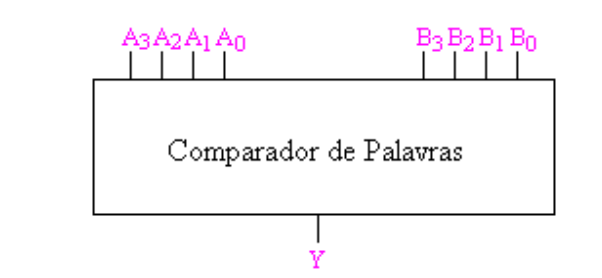
\includegraphics[width=.5\textwidth]{cc1.png}	
\end{figure}

Um comparador tem como saída 1 se os comprimentos forem iguais,caso
contrário a saída sera 0.
Ele também pode possuir três saídas:

\begin{itemize}
	\item	se A=B
	\item	se A\textless B
	\item	se A\textgreater B
\end{itemize}

Para uma boa realização de um circuito combinacional é necessário seguir alguns
passos,como os mostrados abaixo:

\begin{enumerate}[label=(\alph*)]
	\item	Descrever sistema;
	\item 	Elaborar tabela da verdade;
	\item	Obter funções booleanas a partir da tabela verdade;
	\item	Simplificar funções booleanas obtidas ;
	\item	Elaborar diagrama lógico.
\end{enumerate}
Dessa maneira, fica mais intuitivo a realização da montagem e análise do circuito.

\section{Procedimentos}
\label{sec:Procedimentos}
\subsection{Parte 1}
\begin{enumerate}[label=(\roman*)]
	\item Complete a tabela da verdade abaixo do circuito XNOR e obtenha a sua função booleana Zi .
	\item Modifique a função Zi obtida no item a de forma a usar apenas portas NAND de 2 entradas.
	\item Desenhe, como um subcircuito, o diagrama lógico parcial da comparação do par de bits (Ai ,
	Bi ), realize a simulação funcional e verifique a tabela da verdade do item a.
	\item Desenhe o circuito total e faça a simulação funcional do diagrama lógico total, verificando a
	tabela verdade obtida.
	\item Realize a simulação temporal do circuito e comente os resultados obtidos justificando-os.
\end{enumerate}
\subsection{Parte 2}
\begin{enumerate}[label=(\roman*)]
	\item Elabore a tabela da verdade parcial e obtenha as funções booleanas parciais do circuito
	Comparador de 1 bit.
	\item Minimize as expressões obtidas no item a.
	\item Desenhe o subcircuito e faça a simulação funcional do diagrama lógico parcial do
	Comparador de 1 bit, comparando com a tabela verdade do item a.
	\item Desenhe o circuito e realize a simulação funcional do diagrama lógico total do Comparador
	de 2 bits, escrevendo a tabela verdade obtida.
	\item Realize a simulação temporal do circuito do Comparador de 2 bits e comente os resultados.
\end{enumerate}

\section{Análise dos Resultados}
\label{sec:Resultados}
\subsection{Analise: Parte 1}

A partir da tabela verdade~\ref{tab:XNOR} obtivemos a equação para montar o circuito comparador de 1 bit.
\begin{table}[H]
	\centering
	\caption{Tabela XNOR(Comparador de 1 bit)}
	\begin{tabular}{|c|c|c|}
		\hline
		\multicolumn{1}{|c}{A} & \multicolumn{1}{|c|}{B} & \multicolumn{1}{c|}{Zi}\\
		\hline
		0 & 0 & 1\\
		0 & 1 & 0\\
		1 & 0 & 0\\
		1 & 1 & 1\\
		\hline
	\end{tabular}
	\label{tab:XNOR}
\end{table}
Com a simplificação da tabela~\ref{tab:XNOR} obtivemos a seguinte equação: 
\begin{figure}[H]
	\centering
	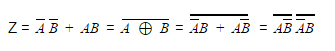
\includegraphics[width=.5\textwidth]{simpxnor.png}
	\label{fig:simpxnor}	
\end{figure}
O diagrama da função encontrada está representado na figura~\ref{fig:dlc1} abaixo:
\begin{figure}[H]
	\centering
	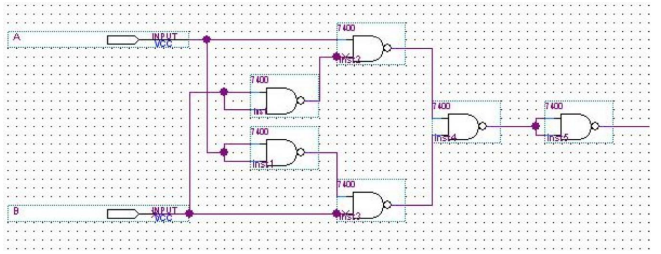
\includegraphics[width=.5\textwidth]{dlc1bit.png}
	\caption{Diagrama Lógico do Comparador de 1 bit}
	\label{fig:dlc1}	
\end{figure}
Já um comparador de 3 bits pode ser implementado pela figura~\ref{fig:cc3b}:
\begin{figure}[H]
	\centering
	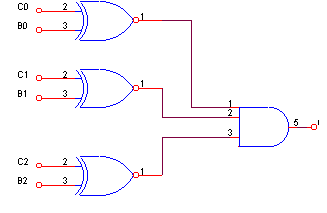
\includegraphics[width=.5\textwidth]{cc3bitex.png}
	\caption{Circuito Comparador de 3 bits.}
	\label{fig:cc3b}
\end{figure}
Como no experimento é pedido apenas com portas NAND, o circuito,na figura~\ref{fig:dtc3} e sua wave form na figura~\ref{fig:wf3}, foi implementado da seguinte maneira:
\begin{figure}[H]
	\centering
	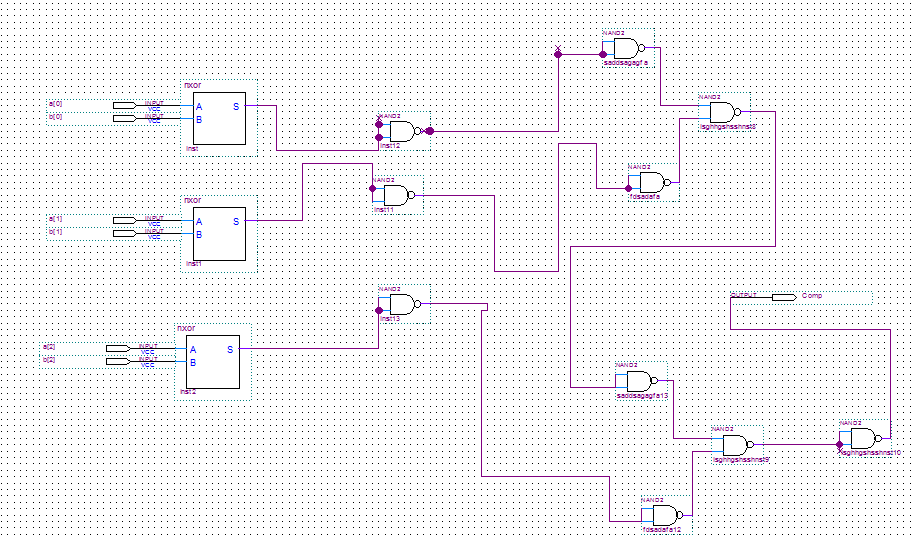
\includegraphics[width=.5\textwidth]{dtcc3bits.png}
	\caption{Diagrama total do Circuito comparador de 3 bits}
	\label{fig:dtc3}
\end{figure}

\begin{figure}[H]
	\centering
	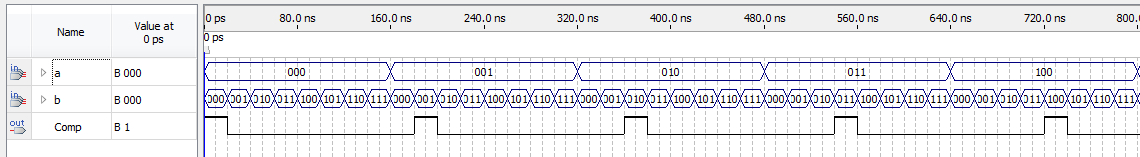
\includegraphics[width=.5\textwidth]{wfcc3bits.png}
	\caption{Forma de onda do circuito comparador de 3 bits}
	\label{fig:wf3}
\end{figure}

\subsection{Analise: Parte 2}

Preenchendo-se a tabela verdade parcial do comparador de 1 bit, tal que  Y1 = 1  \textless-\textgreater A\textgreater B, Y2 = 1 \textless-\textgreater  A=B e Y3 = 1 \textless-\textgreater A\textless B, obtivemos a equação necessária para montar o circuito comparador de igualdade, minoridade e maioridade de 1 bit.

\begin{table}[H]
	\centering
	\caption{Comparador de 1 bit}
	\begin{tabular}{|c|c|c|c|c|}
		\hline
		\multicolumn{1}{|c|}{A} & \multicolumn{1}{|c|}{B} & \multicolumn{1}{|c|}{Y1=\textgreater A\textgreater B} & \multicolumn{1}{|c|}{Y2=\textgreater A=B} & \multicolumn{1}{|c|}{Y3=\textgreater A\textless B} \\
		\hline
		0 & 0 & 0 & 1 & 0\\
		0 & 1 & 0 & 0 & 1\\
		1 & 0 & 1 & 0 & 0\\
		1 & 1 & 0 & 1 & 0\\
		\hline
	\end{tabular}
	\label{tab:c1b}
\end{table}

Sendo,
\begin{figure}[H]
	\centering
	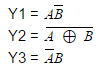
\includegraphics[width=.2\textwidth]{p2el.png}
\end{figure}

Através de Y1,Y2 e Y3, montamos o circuito comparador de 1 bit, como mostrado na figura~\ref{fig:cc1} abaixo:
\begin{figure}[H]
	\centering
	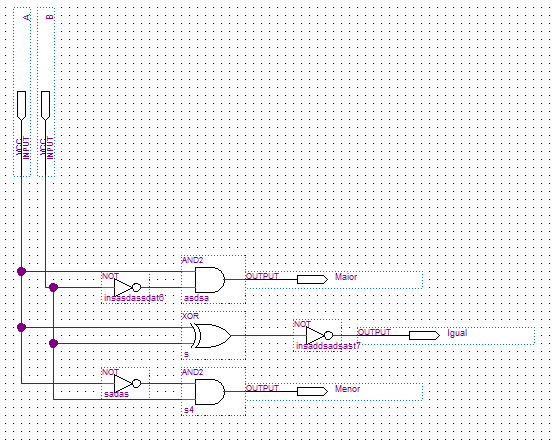
\includegraphics[width=.7\textwidth]{cc1bit2.png}
	\caption{Circuito Comparador de 1 bit}
	\label{fig:cc1}
\end{figure}

E, finalmente, utilizando o comparador de 1 bit, implementamos o circuito comparador de 2 bits representados pelas figuras~\ref{fig:cc2} e~\ref{fig:wf2}:

\begin{figure}[H]
	\centering
	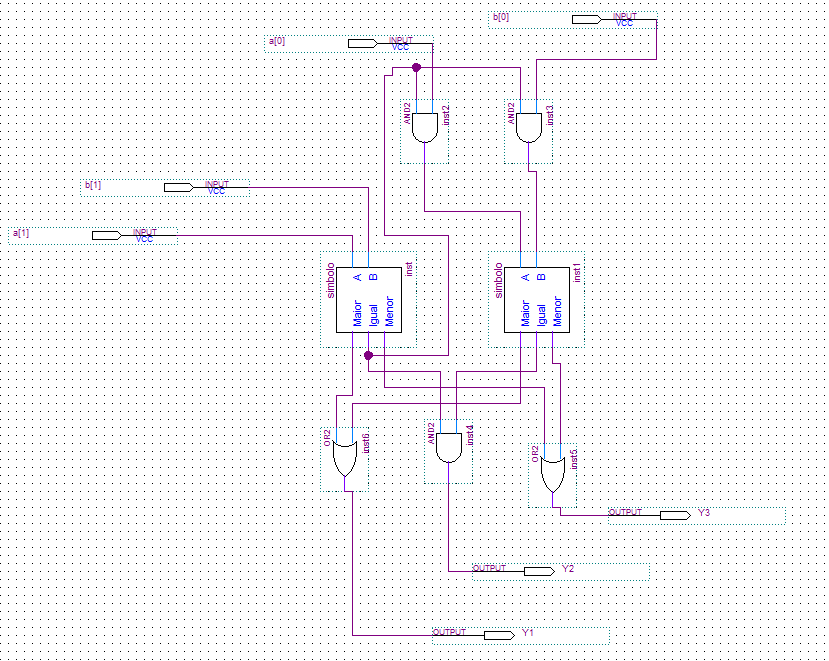
\includegraphics[width=.7\textwidth]{cc2b.png}
	\caption{Circuito Comparador de 2 bit}
	\label{fig:cc2}
\end{figure}
\begin{figure}[H]
	\centering
	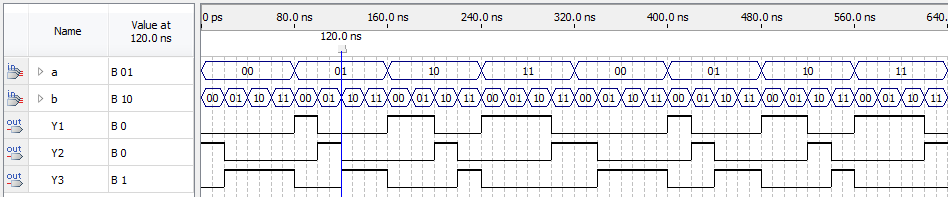
\includegraphics[width=.7\textwidth]{wf2b.png}
	\caption{Wave Form do Comparador de 2 bit}
	\label{fig:wf2}
\end{figure}

\section{Conclusão}
\label{sec:Conclusao}
Foi estudado nesse relatório o uso de comparadores de bits, bem como o uso da
ferramenta Quartus II para a implementação de circuitos. Foram usados métodos
conhecidos da síntese de circuitos combinacionais já vistos em aulas teóricas.
Pode-se afirmar que, com a semelhança dos resultados nas tabelas verdades com
as tabelas do Quartus II que foi um experimento de bastante sucesso.
\newpage 
% Colocar aqui apenas as respostas dos itens da Auto-Avaliação
\section*{Auto-Avaliação}

\begin{enumerate}
    \item b
    \item d
    \item d
    \item b
    \item b
\end{enumerate}


\end{document}